\chapter{Presentaciones}
\label{cha:presentaciones}

\begin{enestecapitulo}
	\item[\emoji{fearful-face}] Cómo domar el pánico escénico al hablar en público.
	\item[\emoji{building-construction}] Construir un discurso que atrape a tu audiencia en treinta segundos.
	\item[\emoji{bar-chart}] Diseñar gráficos honestos que comuniquen tus datos sin mentir.
	\item[\emoji{desktop-computer}] Dominar herramientas digitales para controlar tu presentación.
	\item[\emoji{electric-plug}] Sobrevivir al proyector rebelde.
	\item[\emoji{rocket}] Llevar tus presentaciones más allá del aula.
\end{enestecapitulo}

En los capítulos anteriores recorrimos la historia de la ciencia, discutimos cómo los filósofos intentan definirla y aprendimos cómo los científicos publican sus hallazgos en revistas especializadas.
Pero hay un abismo entre \emph{escribir} ciencia y \emph{presentarla} en público.
Y ese abismo tiene nombre: el terror escénico.

Puedes resolver ecuaciones diferenciales mientras desayunas, demostrar teoremas por inducción, escribir un compilador desde cero y recitar de memoria las leyes de la termodinámica, pero basta que tu profesor diga las fatídicas palabras \emph{“la siguiente clase expone su equipo”} para que tu sistema nervioso colapse.

¿Por qué nos aterra tanto hablar en público?
¿Existe una forma correcta de preparar una exposición científica?
¿Realmente importa cómo se ven las diapositivas o basta con que “los datos hablen por sí solos”?
Y si todo sale mal, ¿hay manera de salvar la presentación frente al proyector que parpadea y el cable VGA que se resiste a cooperar?

Este capítulo está dedicado a responder esas preguntas.
No es un recetario de autoayuda ni un manual de oratoria para ejecutivos trajeados: es una guía de supervivencia práctica para estudiantes universitarios que, como tú, prefieren aulas o laboratorios antes que los escenarios, pero que inevitablemente tendrán que enfrentarse a una audiencia el día del examen o la defensa de su proyecto final.

\begin{digress}{Los datos no hablan}
	Existe una creencia casi religiosa entre los estudiantes de ciencias: \emph{los datos hablarán por sí solos}.
	Es una idea hermosa, poética incluso, pero rotundamente falsa.
	Las hojas de cálculo no tienen cuerdas vocales.
	Un gráfico de dispersión no se para frente al público y dice “miren qué tendencia tan interesante”.
	Toda comunicación está centrada en la audiencia, y si tú no haces el esfuerzo de traducir tus datos a lenguaje humano, nadie más lo hará.
\end{digress}

\section{La fisiología del terror escénico}
\label{sec:fisiologiaterror}

Antes de hablar de diapositivas, fuentes tipográficas o atajos de teclado, tenemos que hablar de lo que te ocurre \emph{por dentro} cuando te paras frente a una audiencia.
No importa qué tan bien diseñada esté tu presentación si tu cerebro está en modo \emph{huida} y tus manos tiemblan tanto que no puedes sostener el apuntador láser.

El miedo a hablar en público tiene nombre clínico: \terminology{glosofobia}.
Y no, no es un defecto de carácter ni una señal de que eres un mal estudiante.
Es una respuesta evolutiva perfectamente normal que, desafortunadamente, no distingue entre un tigre dientes de sable y un salón lleno de compañeros de clase.

\subsection*{El mecanismo de lucha o huida}

Cuando caminas hacia el frente del salón, tu cerebro primitivo interpreta las docenas de miradas fijas y expectantes con el mismo código de alarma que usaban tus ancestros en la sabana africana.
¿Por qué?
La psicología evolutiva ofrece una explicación tan fascinante como perturbadora: para un homínido del Pleistoceno, ser rechazado por su tribu no era simplemente incómodo —era una sentencia de muerte \cite{Baumeister1995}.
Sin el grupo, no había protección contra depredadores, ni acceso a alimento compartido, ni posibilidad de reproducirse.
El ostracismo social y la muerte eran, en la práctica, la misma cosa.

\begin{figure}
	\centering
	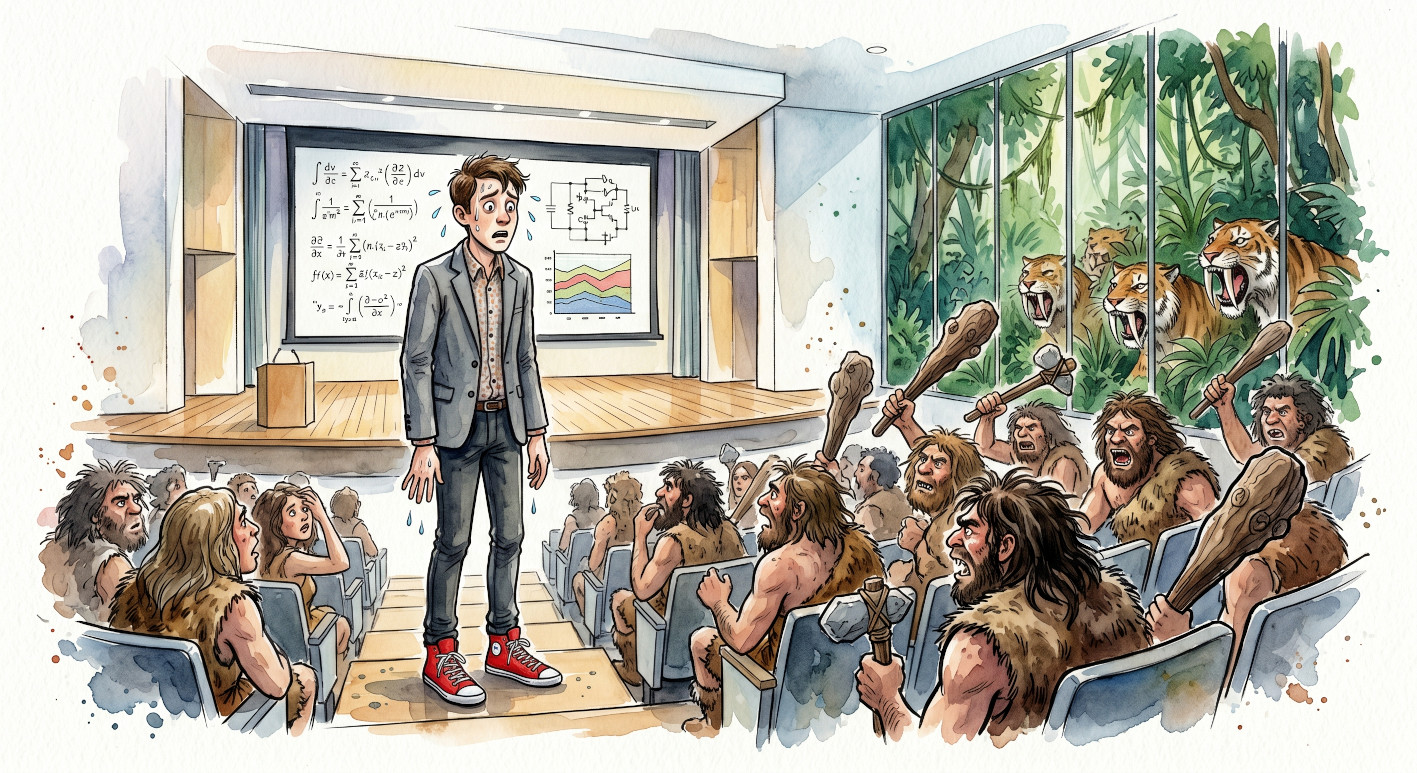
\includegraphics[width=0.8\textwidth]{img/glosofobia}
	\caption{El origen evolutivo del pánico escénico: si dices algo malo, te expulsan de la tribu, y sin tribu, estás a merced de los tigres.}
\end{figure}

Por eso evolucionamos con un sistema de alarma hipersensible a la evaluación social negativa: el ridículo, el juicio ajeno y la desaprobación del grupo se procesan en el cerebro como amenazas existenciales.
Cuando te paras a exponer, tu amígdala no está viendo a tu profesor de Matemáticas Discretas con su termo de café; está viendo a treinta pares de ojos que podrían expulsarte de la tribu y dejarte a merced de los tigres.
El resultado es una cascada bioquímica implacable: las glándulas suprarrenales liberan cortisol y adrenalina, el ritmo cardíaco se dispara, la respiración se vuelve superficial y acelerada, las manos tiemblan, la boca se seca, y en casos severos aparecen náuseas y sudoración profusa.

Lo irónico del asunto es que esta inyección hormonal, diseñada para ayudarte a huir de un depredador, resulta completamente inútil —y activamente contraproducente— cuando lo que necesitas es explicar la complejidad asintótica de un algoritmo frente a tu profesor de Matemáticas Discretas.

\begin{remember}
	\label{rem:glosofobia}
	La \terminology{glosofobia} es el miedo irracional a hablar en público.
	Se trata de una respuesta psicofisiológica en la que la amígdala cerebral interpreta la atención de la audiencia como una amenaza existencial, desencadenando la respuesta de lucha o huida.
	No es una debilidad: es biología.
\end{remember}

\subsection*{La paradoja del pánico: por qué combatirlo lo empeora}

Aquí viene la parte contraintuitiva: el esfuerzo consciente por reprimir o esconder la ansiedad suele exacerbarla.
Es como cuando alguien te dice “no pienses en un elefante rosa” y es justo en lo único que puedes pensar.
Los expertos en comunicación coinciden en que la estrategia ganadora no es luchar contra el nerviosismo, sino aceptarlo \cite{Hennessey2019, Anderson2016}.

Piénsalo así: cuando admites frente a tu audiencia que estás un poco nervioso, con una leve sonrisa y sin dramatizar, ocurre algo casi mágico.
El público, que también ha pasado por lo mismo, inmediatamente se relaja y te perdona el temblor en la voz.
Como explica Chris Anderson, curador de las célebres conferencias TED, en su guía oficial de oratoria \cite{Anderson2016}, mostrar vulnerabilidad es como cuando un vaquero entra a la cantina del pueblo y abre su abrigo para mostrar que no lleva armas: todos se relajan al instante.
De la misma forma, admitir tu nerviosismo es un acto de confianza que humaniza tu presentación y crea una conexión genuina con la audiencia.

\begin{digress}{La respiración que te salva}
	Hay una herramienta que tienes disponible en todo momento y que interviene directamente sobre tu sistema nervioso: la respiración diafragmática.
	Cuando fuerzas exhalaciones lentas y controladas, envías una señal neuroquímica a tu cerebro indicando que la amenaza ha pasado.
	Literalmente le dices a tu cuerpo: “tranquilo, no hay tigres aquí”.
	La próxima vez que sientas el pánico subir antes de una exposición, haz tres exhalaciones profundas.
	Funciona incluso cuando ya estás frente al público y sientes que la voz te tiembla.
\end{digress}

\section{La arquitectura del discurso}
\label{sec:arquitecturadiscurso}

Una vez que has domado la tormenta bioquímica y tu ritmo cardíaco ha descendido a niveles compatibles con el pensamiento racional, llega el momento de construir tu narrativa.
Y aquí ocurre la tragedia más frecuente en las facultades de ciencias.

El estudiante asume, con una inocencia entrañable pero letal, que el público comparte su mismo nivel de obsesión por los minúsculos detalles metodológicos que lo han mantenido despierto durante meses.
Sube al atril y suelta un torrente de jerga técnica incomprensible, convencido de que la mera transferencia de datos crudos constituye una exposición exitosa.

La cruda realidad es que la atención humana es un recurso escaso, frágil y altamente volátil.
Antes de sembrar una idea compleja en la mente de otra persona, necesitas ganarte su permiso y su confianza.

\subsection*{El \emph{discurso de ascensor}: los primeros treinta segundos}

En el implacable mundo de la comunicación académica, dispones de una ventana crítica de entre treinta y sesenta segundos para justificar la existencia misma de tu exposición.
A esta técnica se le conoce como \terminology[discurso de ascensor]{discurso de ascensor} (\emph{elevator pitch} en inglés), y la premisa es draconiana: si no logras capturar la atención de tu audiencia en ese lapso, la perdiste para siempre.

Piensa en lo que pasa por la cabeza de tus compañeros y profesores cuando te paras frente a ellos.
Quizás están pensando en el examen de la siguiente hora.
Quizás están calculando mentalmente a qué hora deben salir del campus para alcanzar la Ruta 1 o la Ruta 13 hacia el centro de Cuernavaca.
Quizás simplemente tienen hambre.
Tu misión es sacarlos de ese ensimismamiento con un gancho intelectual irresistible.

Un \emph{discurso de ascensor} efectivo responde, en menos de un minuto, a cuatro preguntas fundamentales:

\begin{description}
	\item[¿Cuál es el problema?] Empieza con el dolor, la falla o el misterio universal que justifica tu investigación.
	\item[¿Cuál es tu enfoque?] Describe a grandes rasgos tu metodología o hipótesis, sin jerga innecesaria.
	\item[¿Por qué debería importarle a la audiencia?] Responde al temido \emph{“¿y qué?”} de todo evaluador académico.
	\item[¿Por qué eres tú la persona indicada para resolverlo?] Afirma sutilmente tu competencia sin caer en la arrogancia.
\end{description}

\begin{remember}
	\label{rem:elevatorpitch}
	El \terminology{discurso de ascensor} es una técnica de comunicación que consiste en condensar la esencia de una investigación en un mensaje de treinta a sesenta segundos, respondiendo qué problema resuelve, cómo lo aborda, por qué es relevante y qué credibilidad tiene quien lo presenta.
\end{remember}

\subsection*{La línea conductora}

Más allá del gancho inicial, toda buena presentación tiene lo que Anderson denomina un \emph{throughline} \cite{Anderson2016}: un hilo conductor que conecta todas las secciones, los datos empíricos y los apoyos visuales en un marco coherente y unificado.

Un error clásico es confundir el \emph{tema} con la \emph{idea central}.
El tema es un sustantivo inerte: “Estudio del problema del agente viajero en grafos dirigidos”.
La idea central es una revelación dinámica: “Por qué encontrar la ruta más corta se vuelve imposible cuando añades más ciudades”.

La regla es espartana: esta idea central debe poder encapsularse en un máximo de quince palabras, y debe poseer un ángulo intrigante.
Una vez definida, debes someter tu presentación a una auditoría de descarte despiadada.
Cada diapositiva, cada gráfica, cada anécdota debe anclarse a este pilar narrativo.
Lo que no sume directamente a la línea conductora, aunque te haya costado horas de laboratorio, debe ir a la papelera.

\begin{remember}
	\label{rem:throughline}
	La \terminology{línea conductora} (\emph{throughline}) es la idea central que conecta todos los elementos de una presentación.
	Debe ser concisa (máximo quince palabras), intrigante y servir como filtro implacable: lo que no la refuerce, sobra.
\end{remember}

\subsection*{La ecuación de Marshall: cómo hablar de ciencia}

La física y comunicadora Melissa Marshall ha dedicado su carrera a enseñarle a científicos e ingenieros a hablar con el resto de la humanidad.
Su principio fundamental es que se debe reemplazar la jerga académica por historias vívidas, ejemplos tangibles y analogías terrenales, pero sin caer jamás en la condescendencia o en la simplificación que distorsione la verdad científica.

Marshall propone una ecuación heurística que resume, con ironía y precisión, la receta para que una audiencia te entienda \cite{Marshall2012}:

\begin{align*}
	\textit{Comprensión} = \frac{\textit{Ciencia} - \textit{Jerga} - \textit{Viñetas}}{\textit{Relevancia}} \times \textit{Pasión}
\end{align*}

Traducida al español llano: el nivel de comprensión de tu audiencia es directamente proporcional al contenido científico, \emph{siempre y cuando} le restes implacablemente los tecnicismos innecesarios (que sólo inflan tu ego) y las aburridas listas de viñetas (que anestesian el nervio óptico).
Ese valor purificado lo divides por la relevancia que el tema tiene para el espectador —porque si al público no le importa, no te va a entender— y finalmente lo multiplicas por la pasión genuina que proyectas al hablar.

La moraleja es doble: simplifica sin distorsionar y contagia tu entusiasmo.
Si a ti no te emociona tu propia investigación, ¿por qué debería emocionarle a alguien más?

\section{Estética de la información}
\label{sec:esteticatufte}

Habiendo estructurado tu narrativa con el rigor de un arquitecto, llega el momento de representar visualmente tus datos.
Y aquí, querido lector, se cometen crímenes de lesa humanidad informativa.

Con el pretexto de que un gráfico debe lucir “atractivo” o “moderno”, el estudiante promedio abre su hoja de cálculo favorita y produce aberraciones tridimensionales con sombras, degradados arcoíris y efectos de bisel que harían llorar a cualquier diseñador profesional.

El estadístico Edward Tufte, profesor emérito de la Universidad de Yale, consagró su carrera a combatir esta epidemia en su obra clásica \emph{The Visual Display of Quantitative Information} \cite{Tufte1983}.
Su postulado fundamental es implacable: \emph{el desorden y la confusión son fallas del diseño, no atributos de la información}.

\subsection*{La proporción de tinta de datos}

Tufte introdujo una métrica brutalmente simple para evaluar la calidad de un gráfico: la \terminology[Data-Ink Ratio]{proporción de tinta de datos} (\emph{Data-Ink Ratio}), es decir, la proporción de tinta dedicada a los datos:

\begin{align*}
	\textit{Data-Ink Ratio} = \frac{\textit{Tinta que representa datos}}{\textit{Tinta total usada en el gráfico}}
\end{align*}

En la práctica, la “tinta” son los píxeles que iluminas en la pantalla del proyector.
La meta es maximizar esta proporción, buscando un valor lo más cercano posible a \(1.0\).
En un gráfico con una proporción de tinta de datos de \(1.0\), cada píxel encendido representa un dato real.
Si borras un solo punto, pierdes información.
Todo lo demás —sombras, degradados, bordes gruesos, cuadrículas estridentes, íconos decorativos— es lo que Tufte bautizó como \terminology[Chartjunk]{basura gráfica} (\emph{chartjunk}).

\begin{remember}
	\label{rem:datainkratio}
	El \terminology{proporción de tinta de datos} mide la eficiencia de un gráfico: cuánto de lo que muestras es información genuina versus decoración superflua.
	La regla de oro: maximiza la tinta de datos, elimina la \terminology{basura gráfica}.
\end{remember}

\subsection*{Auditoría de descarte visual}

Para purificar tus gráficos según los estándares de Tufte, aplica esta lista de verificación sin piedad:

\begin{description}
	\item[Destruye el 3D falso.] Nunca uses la tercera dimensión para representar datos de una o dos dimensiones.
	      Un gráfico de pastel en 3D distorsiona las proporciones por la perspectiva y convierte tus porcentajes en mentiras visuales.
	\item[Mutila sombreados y degradados.] Usa colores sólidos.
	      Las sombras paralelas y los degradados añaden ruido óptico que compite con tus datos.
	\item[Suaviza o elimina las cuadrículas.] Si son indispensables para leer valores, reduce su grosor y cambia su color a un gris tan tenue que casi desaparezca.
	\item[Suprime los bordes del gráfico.] Las cajas cerradas son innecesarias.
	      Deja que el espacio en blanco actúe como delimitador natural.
	\item[Etiqueta directamente las series.] Las leyendas flotantes obligan al ojo a un constante ping-pong entre el gráfico y el recuadro.
	      Escribe la etiqueta junto a la curva o barra correspondiente.
\end{description}

\subsection*{Integridad gráfica y el factor de engaño}

La visualización científica no es sólo una cuestión de estética: es una cuestión de honestidad ética.
Tufte propuso el \terminology{Factor de Engaño} (\emph{Lie Factor}) para medir cuantitativamente la veracidad de un gráfico:

\begin{align*}
	\textit{Factor de Engaño} = \frac{\textit{Tamaño del efecto mostrado en el gráfico}}{\textit{Tamaño del efecto real en los datos}}
\end{align*}

Un gráfico honesto tiene un \emph{Factor de Engaño} de \(1.0\).
Si el valor se aleja significativamente de \(1.0\), tu gráfico le está mintiendo a la audiencia.

Hay dos trampas recurrentes en las presentaciones universitarias: truncar el eje Y para exagerar diferencias minúsculas entre dos barras (lo que amplifica visualmente un cambio insignificante), y representar datos unidimensionales con áreas o volúmenes (donde un valor que se duplica se dibuja como un círculo de \emph{diámetro} doble, lo que cuadruplica el \emph{área} percibida).
La regla de oro es simple: tú no elegiste dedicarte a la ciencia para contar mentiras.
Tus gráficos tampoco deberían hacerlo.

\begin{remember}
	\label{rem:integrity}
	El \terminology{Factor de Engaño} (\emph{Lie Factor}) cuantifica la honestidad visual de un gráfico.
	Un valor de \(1.0\) indica veracidad absoluta.
	Truncar ejes o inflar dimensiones no es diseño creativo: es deshonestidad intelectual.
\end{remember}

\section{El dominio del escenario digital}
\label{sec:escenariodigital}

Llegamos al momento de la verdad: estás frente a la computadora del aula, tu presentación está lista y tus datos son impecables.
Pero hay una diferencia abismal entre darle click a la flecha de avance como un autómata y dominar el escenario como un director de orquesta.

\subsection*{Google Slides como panel de control}

Hoy en día, plataformas como Google Slides se han convertido en el estándar de facto en el ámbito universitario: son gratuitas, colaborativas y accesibles desde cualquier navegador.
Dicho esto, son también el ejemplo perfecto de una herramienta cuyo potencial permanece virgen en el 95\% de las computadoras del campus.

La mayoría de los estudiantes usan Google Slides como quien usa un Ferrari para ir a la esquina: le pican a la flecha de avanzar y a la de retroceder, y creen que ya dominan el arte.
Es como tener una navaja suiza y usar únicamente la uña para abrir botellas.

Los atajos de teclado que vienen a continuación son las herramientas que separan al aficionado del profesional:

\begin{description}
	\item[Pantalla negra (tecla \texttt{B} o \texttt{.}):] Apaga el proyector momentáneamente.
	      Obliga a la audiencia a desviar la mirada de la pantalla y centrar su atención absoluta en \emph{ti}.
	      Es el recurso táctico más subestimado y poderoso del arsenal del presentador.
	\item[Pantalla blanca (tecla \texttt{W} o \texttt{,}):] Similar a la pantalla negra, pero útil en salones muy iluminados donde un apagón súbito resultaría discordante.
	\item[Vista del presentador (\texttt{Ctrl+Alt+Shift+S}):] Abre una consola privada donde puedes ver tus notas, controlar el cronómetro y previsualizar la siguiente diapositiva, todo sin que la audiencia se entere.
	\item[Apuntador láser virtual (\texttt{L}):] Convierte el cursor en un trazo láser rojo para señalar puntos en gráficas sin necesidad de un periférico externo.
	\item[Subtítulos en tiempo real (\texttt{Ctrl+Shift+C}):] Activa la transcripción automática de tus palabras.
	      Una herramienta de accesibilidad que además te obliga a vocalizar con claridad.
\end{description}

\begin{remember}
	\label{rem:atajos}
	La tecla \texttt{B} (pantalla negra) es el arma secreta del buen presentador.
	Cuando la pantalla se apaga, los ojos de la audiencia —esos mismos que segundos antes revisaban el WhatsApp debajo de la butaca— se ven forzados a buscarte a ti, la única fuente de información que queda en la sala.
	Es un acto de autoridad escénica sutil pero devastadoramente efectivo.
\end{remember}

\subsection*{El mito de la improvisación}

Existe una creencia peligrosa en los pasillos de las facultades de ciencias: que un dominio profundo del tema te exime de la necesidad de ensayar.
La historia de la academia demuestra que esto es categóricamente falso.

La improvisación técnica, bajo los efectos de la adrenalina escénica, suele derivar en digresiones interminables, muletillas verbales crónicas y la pérdida total del hilo conductor.
Pero ensayar no significa memorizar un guion palabra por palabra como si fueras un loro académico.
Memorizar de manera robótica destruye la ilusión de conversación y aniquila la conexión visual con la audiencia.

El verdadero ensayo consiste en familiarizarte con la \emph{coreografía de las ideas}: saber en qué momento hacer una pausa para que un concepto pesado decante, cuándo subir el volumen para enfatizar un hallazgo, y cuándo contar esa anécdota del laboratorio que humaniza tus datos.
Como dice el proverbio moderno de la oratoria: \emph{la práctica no busca la perfección inalcanzable; la práctica hace que la imperfección sea llevadera}.

\section{La trinchera tecnológica}
\label{sec:trincheratecnologica}

Toda la preparación psicológica, la estructura narrativa impecable y el dominio de Google Slides pueden desmoronarse en los fatídicos cinco minutos previos a tu exposición por culpa de un enemigo silencioso y terriblemente terco: el hardware del aula universitaria.

La infraestructura educativa en las universidades públicas latinoamericanas existe en un fascinante estado de superposición histórica: en el mismo metro cuadrado conviven proyectores recién instalados con cableado VGA que data de la época en que los monitores CRT dominaban la Tierra.

\subsection*{VGA, HDMI y otros especímenes del ecosistema}

El conocimiento íntimo de los protocolos de transmisión de video es un requisito ineludible para el orador contemporáneo.
Ignorar esta realidad es un acto de negligencia académica que te pasará factura en el peor momento posible.

\begin{description}
	\item[VGA (Video Graphics Array):] El gran veterano de quince pines azules.
	      Omnipresente en instalaciones que no han renovado su infraestructura desde el siglo pasado.
	      Transmite señal \emph{analógica} —y sólo video— por lo que necesitas un cable de audio auxiliar aparte si tu presentación incluye sonido.
	      Un VGA maltratado por generaciones de estudiantes proyectará tu impecable gráfica de datos con un deprimente tinte verdoso o rosado.
	\item[HDMI (High-Definition Multimedia Interface):] El estándar digital contemporáneo.
	      Transmite video y audio de alta definición por un solo cable.
	      Pero es mecánicamente frágil: los puertos empotrados en la pared del salón sufren falsos contactos y misteriosos problemas de \emph{handshake} digital que impiden la sincronización.
	\item[USB-C / DisplayPort:] El presente y el futuro, común en laptops modernas y ultrafinas.
	      Los proyectores universitarios rara vez tienen este puerto de forma nativa, así que dependen de la magia oscura de los adaptadores externos (\emph{dongles}).
\end{description}

\begin{remember}
	\label{rem:dongle}
	La ley de hierro del presentador universitario: jamás asumas que el salón tendrá el adaptador que necesitas.
	La probabilidad de que el cable que requieres esté disponible es inversamente proporcional a la importancia de tu presentación.
	Carga siempre tu propio arsenal de \emph{dongles} en la mochila, como quien lleva un botiquín de primeros auxilios a una excursión por la selva.
\end{remember}

\subsection*{Cuando el audio no suena donde debería}

Un clásico de las exposiciones modernas, y una fuente inagotable de momentos incómodamente hilarantes para la audiencia: conectas tu laptop al panel HDMI del salón, el proyector muestra tus diapositivas en todo su esplendor\ldots{} pero al reproducir ese video demostrativo de tu práctica de laboratorio, el audio sigue saliendo por los minúsculos altavoces de tu computadora, como un murmullo distante que sólo tú y la primera fila pueden escuchar.

En ese instante, verás al profesor inclinar la cabeza como un perro que no entiende de dónde viene el sonido, mientras tú finges que todo está bajo control.

Esto ocurre porque el sistema operativo no ha redirigido automáticamente la salida de audio al nuevo dispositivo.
La solución requiere compostura bajo presión:

\begin{itemize}
	\item En Windows: ve a “Dispositivos de reproducción de audio”, identifica el proyector o panel externo (a veces etiquetado crípticamente como “Intel Display Audio” o con el nombre de la marca del sistema de automatización) y selecciónalo como dispositivo predeterminado.
	\item En macOS: abre “Configuración del Sistema”, navega a “Sonido”, ve a la pestaña “Salida” y selecciona el dispositivo HDMI correspondiente.
\end{itemize}

\subsection*{Protocolo de emergencia: cuando el proyector dice “No Signal”}

Si después de conectar todos los cables correctamente, el proyector enciende sus ventiladores pero sentencia en letras azules el temido “Sin señal”, respira hondo y ejecuta esta lista de diagnóstico como si estuvieras depurando un experimento en el laboratorio:

\begin{enumerate}
	\item Conecta primero el cable al adaptador, y \emph{luego} el ensamble completo a la computadora.
	      Hacerlo al revés puede confundir a la placa base.
	      Si ya cometiste el error, desconecta todo, respira dos segundos y vuelve a conectar en el orden correcto.
	\item Verifica que tu computadora esté duplicando la pantalla y no extendiendo el escritorio (en Windows: \texttt{Windows + P} y selecciona “Duplicar”; en macOS: “Configuración del Sistema” \(\to\) “Pantallas” y activa la opción de reflejar).
	\item Localiza la tecla de función de video (generalmente \texttt{F8} o la que tenga el ícono de un monitor) y presiónala junto con la tecla \texttt{Fn}.
\end{enumerate}

\begin{digress}{El orden de los factores}
	Hay una peculiaridad casi supersticiosa en la electrónica digital: cuando usas adaptadores externos, el orden de conexión sí altera el producto.
	Conecta primero el cable de video al adaptador, y \emph{después} enchufa el ensamble al puerto USB-C de tu laptop.
	Si lo haces al revés, el controlador de video puede no detectar el cambio de capacitancia en el puerto, asumiendo que no hay nada conectado.
	La cura es simple: desconecta, respira hondo dos segundos, y vuelve a conectar en el orden correcto.
\end{digress}

\section{Referentes de presentaciones}
\label{sec:referentes}

Hasta aquí hemos hablado de principios, reglas y trucos.
Pero nadie mejora su oratoria leyendo solamente tratados teóricos, de la misma forma que nadie aprende a besar con un manual de anatomía.
A continuación, tres referentes —cada uno en un estilo completamente distinto— que demuestran que la comunicación científica puede ser tan emocionante como una película, tan clara como un teorema bien demostrado y tan persuasiva como un argumento filosófico\ldots{} sin necesidad de ponerse traje de ejecutivo ni fingir un entusiasmo que no se siente.

\subsection*{Estadística con un ciclo \texttt{for}}

En su charla \emph{Statistics for Hackers}, presentada en PyCon 2016, \person[VanderPlas]{Jake} propone una idea tan simple como revolucionaria: si sabes escribir un ciclo \texttt{for} en Python, puedes entender estadística\footurl{https://youtu.be/Iq9DzN6mvYA}.

En lugar de abrumar a la audiencia con fórmulas y distribuciones, VanderPlas reemplaza la estadística tradicional basada en pruebas de hipótesis y valores \(p\) por simulaciones computacionales: remuestreo, permutaciones y \emph{bootstrap}.
Muestra cómo un puñado de líneas de código pueden responder preguntas como \emph{¿es significativa la diferencia entre estos dos grupos?} sin necesidad de memorizar tablas ni invocar teoremas.

La lección para tu propia práctica es doble: primera, VanderPlas eligió una \emph{idea central} nítida “la estadística no es difícil si la abordas desde la computación” y no se desvió de ella ni un minuto.
Segunda, llenó la pantalla de código \emph{vivo} que escribía y ejecutaba en tiempo real, aplicando el principio de Tufte al pie de la letra: cada línea de código era tinta de datos, no decoración.

\subsection*{La guerra en datos}

\emph{The Fallen of World War II}, del cineasta \person[Halloran]{Neil}, es un documental animado que cuenta la historia de la Segunda Guerra Mundial usando exclusivamente visualización de datos\footurl{https://youtu.be/DwKPFT-RioU}.

En dieciocho minutos, Halloran transforma cifras —a veces abstractas, a veces insoportablemente concretas— en gráficos animados que muestran el costo humano del conflicto: las bajas militares y civiles, país por país, mes a mes, y cómo esas cifras se comparan con otras guerras en la historia.

Lo que hace magistral esta pieza no es la complejidad de los datos, sino el \emph{ritmo narrativo}.
Halloran no suelta todas las cifras de golpe: dosifica la información, deja que cada revelación respire, y construye un arco emocional que va de la contextualización histórica a un clímax devastador, para terminar con una reflexión sobre la paz en el presente.
Es la demostración definitiva de que los datos, cuando se presentan con pausas, contraste y humanidad, pueden conmover más que cualquier discurso.

\subsection*{El dilema del prisionero explicado con magia}

El canal \emph{Veritasium en español} ofrece un ejemplo perfecto de cómo comunicar un concepto complejo —en este caso, el dilema del prisionero de la teoría de juegos— sin perder rigor ni audiencia\footurl{https://youtu.be/vBgrvVY1jGo}.

El presentador no empieza definiendo matrices de pago ni equilibrios de Nash.
Empieza con un juego de cartas y una pregunta: \emph{¿por qué dos personas racionales, actuando en su propio interés, pueden terminar peor que si cooperaran?}
A partir de ahí, el dilema del prisionero se despliega como un mecanismo explicativo para fenómenos tan dispares como la carrera armamentista nuclear, la evolución de la cooperación en la naturaleza y hasta por qué es tan difícil ponerse de acuerdo para lavar los platos en una casa de estudiantes.

Tres aciertos que puedes robar para tus propias presentaciones: \begin{enumerate}
	\item Empieza con un ejemplo tangible, no con la definición formal.
	\item Muestra que el concepto \emph{sirve para algo}: conecta la teoría con problemas reales que tu audiencia reconoce.
	\item No le tengas miedo a contar una historia —el dilema del prisionero es, en el fondo, un drama entre dos sospechosos en celdas separadas, y así lo presenta el video.
\end{enumerate}

\begin{remember}
	\label{rem:referentes}
	Estudiar grandes presentaciones ajenas es tan importante como ensayar las propias.
	Pregúntate siempre: ¿cuál es la idea central de esta charla?
	¿Cómo maneja el ritmo?
	¿Qué hace con los datos?
	¿Por qué me importa lo que me está contando?
	Si puedes responder esas cuatro preguntas, puedes extraer lecciones de cualquier exposición que admires.
\end{remember}

\section{Más allá del aula}
\label{sec:masalladelaula}

Hemos recorrido un camino largo: desde las profundidades de tu sistema nervioso hasta la jungla de cables y adaptadores del salón de clases.
Pero todo este conocimiento tiene una utilidad que trasciende la calificación del semestre.

El \emph{elevator pitch} que preparaste para tu clase de teoría de la computación es el mismo que usarás cuando te topes con un investigador prominente en un congreso y tengas exactamente treinta segundos para causarle una buena impresión.
La disciplina de eliminar la basura gráfica de tus gráficas es la misma que te permitirá comunicar resultados con claridad en una entrevista de trabajo o en una reunión con colegas de otras disciplinas.
La sangre fría que desarrollaste para diagnosticar un proyector rebelde es la misma que necesitarás cuando el equipo del laboratorio falle en el momento más inoportuno.

La comunicación científica no es un adorno para quedar bien con el jurado: es parte integral del quehacer científico.
Una investigación brillante que nadie entiende es, a efectos prácticos, una investigación que no existe.
Una idea poderosa mal presentada es indistinguible de una idea mediocre.
Y un científico que no sabe comunicar sus hallazgos es como un músico que compone sinfonías pero no sabe tocar ningún instrumento: respetable, quizás, pero profundamente inútil en la práctica.

Así que la próxima vez que te paren frente al proyector, con las manos sudorosas y el corazón acelerado, recuerda: no estás frente a un pelotón de fusilamiento (aunque tu comité evaluador ponga caras de póker profesional).
Estás frente a una audiencia que \emph{quiere} que tengas éxito —aunque sea para irse temprano a su casa—, que quiere aprender algo nuevo, y que en el fondo te respeta por el simple hecho de haberte parado ahí, porque ellos también saben lo que se siente.
Tu trabajo —tu único trabajo— es no interponerte entre tus datos y su curiosidad.

\begin{remember}
	\label{rem:final}
	La comunicación no es un complemento de la ciencia: es parte de la ciencia.
	Los datos no hablan solos.
	Los gráficos no se explican solos.
	Las ideas no se transmiten solas.
	La responsabilidad de que tu conocimiento trascienda es tuya.
\end{remember}

A modo de cierre, y antes de que te enfrentes al escuadrón de fusilamiento académico que es tu comité evaluador o tus compañeros de semestre, aquí tienes un compendio de sugerencias pragmáticas para los minutos previos y el transcurso de tu presentación:

\begin{description}
	\item[Combustible y lubricación:]
	      Come algo ligero aproximadamente una hora antes y bebe agua con antelación.
	      El peor efecto de la adrenalina es que seca la boca y sabotea tu vocalización \cite{Anderson2016}.
	      Además, tener una botella a la mano te permite tomar un sorbo táctico si pierdes el hilo; ese simple acto te regala cinco segundos invaluables para respirar profundo y recuperar la compostura \cite{Hennessey2019}.
	\item[El ancla física:]
	      Si sufres de manoteo incontrolable, sostén un objeto.
	      Un apuntador láser (\emph{clicker}) o una botella sirven como un ancla física que canaliza el movimiento errático de tus extremidades.
	      Asegúrate de sostenerlo con la mano que mantenga tu postura abierta hacia la audiencia \cite{Hennessey2019}.
	\item[Economía de píxeles:]
	      Mantén las presentaciones sobrias y con la menor cantidad de texto posible.
	      Sin importar si expones a las 7:00 a.m. o justo después del almuerzo, bombardear al público con un muro de datos garantiza que se desconecten \cite{Hennessey2019}.
	\item[La táctica de los aliados:]
	      Al subir al frente, busca inmediatamente rostros amables que parezcan receptivos.
	      Al identificar a tres o cuatro de estos “amigos” esparcidos por el salón, dales la charla directamente a ellos alternando la mirada.
	      Esto engañará a tu cerebro, reduciendo la amenaza existencial \cite{Anderson2016}.
	\item[Dosis de humor mesurada:]
	      Una presentación mortalmente seria anestesia al público, pero intentar ser un comediante de \emph{stand-up} es un riesgo innecesario.
	      Usa el humor y anécdotas ligeras como especia, no como el plato principal.
	\item[Desgaste de adrenalina:]
	      Si sientes que el corazón se te va a salir del pecho diez minutos antes de pasar, busca un pasillo vacío y haz algunas flexiones o estiramientos intensos.
	      Al quemar físicamente esa energía primitiva, la calma y la claridad mental regresarán \cite{Anderson2016}.
	\item[Raíces en el escenario:]
	      Planta bien los pies.
	      Evita el movimiento de péndulo o el balanceo nervioso de una pierna a otra, así como caminar sin rumbo de un lado a otro; resulta profundamente cansado y distractor para quien te observa \cite{Anderson2016}.
	\item[El traje de luces:]
	      No dejes la elección de tu ropa para la mañana misma de la presentación.
	      Usar ropa limpia, cómoda y adecuada a la ocasión funge como una armadura psicológica que elevará radicalmente tu confianza \cite{Hennessey2019}.
	\item[Lo técnico al final:]
	      Inicia sin piedad con tu discurso de ascensor y tus resultados principales.
	      Guarda los escabrosos detalles técnicos, el código fuente o las demostraciones formales para el final; de ese modo, sirven como material opcional o munición para la ronda de preguntas.
\end{description}

